\apendice{Estudio experimental}
\section{Cuaderno de Trabajo y Evolución Experimental}
El desarrollo del \textit{software} clínico no ha sido un proceso lineal. Durante la fase de ingeniería, se evaluaron diversas arquitecturas y herramientas que fueron sometidas a pruebas de estrés. En este cuaderno de trabajo se documentan los tres retos técnicos más relevantes del proyecto, detallando tanto las aproximaciones iniciales fallidas como las soluciones definitivas implementadas.

\subsection{Experimento 1: Motor de Procesamiento (\textit{Spark SQL vs Pandas})}
\begin{itemize}
    \item \textbf{Objetivo:} Implementar un motor analítico capaz de procesar y filtrar grandes volúmenes de historiales médicos de forma ágil.
    \item \textbf{Aproximación inicial (Fallida):} En las primeras iteraciones se intentó adaptar \textit{Apache Spark SQL}. Sin embargo, su despliegue en entornos \textit{Windows} resultó ser excesivamente complejo y poco eficiente para este caso de uso. Requería la configuración de dependencias externas pesadas (\textit{Hadoop}, \textit{Java}).
    \item \textbf{Solución y Éxito:} Tras analizar el rendimiento, se pivotó hacia el uso de la librería \textit{Pandas} de \textit{Python}. Esta transición eliminó por completo las dependencias de \textit{Java}, permitiendo un procesamiento vectorial nativo y ultrarrápido, perfectamente adaptado al volumen de datos (\textit{Datasets} de tamaño medio) que maneja la unidad.
\end{itemize}

\subsection{Experimento 2: Optimización de \textit{RAM} y Cumplimiento Normativo (\textit{LOPD})}
\begin{itemize}
    \item \textbf{Objetivo:} Ingestar y procesar múltiples registros anuales manteniendo la fluidez de la aplicación web, evitando la degradación del rendimiento por saturación de la memoria \textit{RAM} y garantizando el estricto cumplimiento de la normativa de protección de datos (\textit{LOPD}).
    
    \item \textbf{Aproximación inicial (Fallida):} Originalmente, para evitar el colapso del sistema, se implementó una arquitectura de almacenamiento temporal. El archivo clínico se escribía físicamente en la carpeta temporal del sistema operativo (\textit{Temp}) para ser leído por el motor de \textit{Pandas} y posteriormente eliminado. Sin embargo, esta estrategia fue auditada y descartada por motivos de seguridad: escribir datos clínicos con identificadores personales en el disco físico supone un riesgo crítico de vulneración de la \textit{LOPD}, ya que un fallo eléctrico o un cierre inesperado del servidor podría dejar archivos residuales expuestos y sin borrar.
    
    \item \textbf{Solución y Éxito:} Se rediseñó el flujo hacia un modelo de procesamiento exclusivo en memoria (\textit{In-Memory Analytics}) aprovechando la arquitectura subyacente del \textit{framework Reflex}. La causa de la lentitud original no era la capacidad del servidor, sino que el sistema intentaba enviar (\textit{serializar}\footnote{Proceso de convertir un objeto o estructura de datos en un formato (como una secuencia de \textit{bytes} o una cadena de texto) que puede ser fácilmente almacenado, transmitido o reconstruido más tarde.}) toda la información bruta al navegador del cliente. La solución técnica consistió en declarar las variables que almacenan los \textit{DataFrames} como variables privadas del \textit{backend} (anteponiendo un guion bajo en su nomenclatura, ej. \texttt{\_dataframes\_memoria}). Esto restringe el volumen de datos exclusivamente a la memoria volátil del servidor aislado, enviando al \textit{frontend} únicamente los resultados matemáticos calculados. Esta optimización resolvió instantáneamente la latencia, eliminó las advertencias del compilador y garantizó la total privacidad de los historiales clínicos.
\end{itemize}

\subsection{Experimento 3: Ciberseguridad, Despliegue y Antivirus}
\begin{itemize}
    \item \textbf{Objetivo:} Lograr un empaquetado del \textit{software} que permitiera una distribución segura, sencilla y universal en los equipos del hospital.
    \item \textbf{Aproximación inicial (Fallida):} 
    \begin{enumerate}
        \item Se desplegó un prototipo funcional en la nube (\textit{Reflex Cloud}). Sin embargo, bajo la recomendación de la tutorización académica, se descartó de inmediato debido a los estrictos protocolos de la \textbf{Ley de Protección de Datos} (\textit{LOPD}), que prohíben subir historiales clínicos a servidores externos.
        \item Se optó por un entorno local empaquetando el código en un archivo ejecutable (\textit{.exe}) mediante \textit{PyInstaller}. Esta vía también fracasó: el Antivirus nativo (\textit{Windows Defender}) identificaba la apertura de puertos locales y el uso de \textit{WebSockets} como una amenaza de red, bloqueando la comunicación entre el \textit{Frontend} y el \textit{Backend}.
        \item Se intentó automatizar el despliegue local mediante archivos de procesamiento por lotes (\textit{scripts .bat} en \textit{Windows}). La intención era ejecutar el entorno de \textit{Python} y levantar el servidor local en el equipo de cada facultativo con un doble clic. No obstante, esta alternativa demostró ser ineficiente y propensa a fallos humanos en el entorno clínico: requería mantener abierta una ventana de terminal de comandos (\textit{CMD}) que los usuarios solían cerrar accidentalmente, provocando la caída inmediata de la aplicación. Además, la ejecución de \textit{scripts} no firmados a menudo era bloqueada por las políticas de seguridad del departamento de informática y mantenía un modelo descentralizado que dificultaba enormemente la actualización y el mantenimiento del \textit{software}.
    \end{enumerate}
    \item \textbf{Solución y Éxito:} Se abandonó la compilación de binarios cerrados y la ejecución local en los ordenadores de la unidad. La solución definitiva consistió en migrar hacia una arquitectura de red centralizada basada en la \textbf{contenerización mediante \textit{Docker}}. Al encapsular la aplicación web, las dependencias y la base de datos relacional en contenedores aislados alojados en el servidor central, el facultativo interactúa con el sistema exclusivamente a través de su navegador web estándar. Esta aproximación elimina por completo las interferencias y falsos positivos de \textit{Windows Defender}, ya que el equipo del usuario final no ejecuta procesos de \textit{Python} en segundo plano ni necesita abrir puertos de comunicación de forma local. Para garantizar el uso autónomo del dispositivo portátil (\textit{Raspberry Pi}) fuera de la red hospitalaria, se implementó un \textit{script} en \textit{Bash} (\textit{.sh}) que orquesta automáticamente el levantamiento de los servidores en el propio dispositivo, logrando un despliegue \textit{Plug \& Play} seguro, robusto y libre de bloqueos.
\end{itemize}

\section{Configuración y Parametrización del Sistema}
En el contexto de esta plataforma de \textit{In-Memory Analytics}, la parametrización no se refiere al ajuste de hiperparámetros de modelos de aprendizaje automático, sino a la configuración de los umbrales críticos del sistema, las reglas de gestión de memoria y las directivas de seguridad. 

La elección de estos valores no ha sido arbitraria, sino que responde a un equilibrio calculado entre las limitaciones de \textit{hardware} del terminal físico, los protocolos clínicos y la normativa legal. A continuación, se detallan los parámetros fundamentales establecidos en el entorno de producción.

\subsection{Límite de Ingesta (Cola \textit{FIFO}: N = 10)}
\begin{itemize}
    \item \textbf{Parámetro:} Capacidad máxima de la cola de archivos/registros cargados simultáneamente en memoria.
    \item \textbf{Valor configurado:} 10 archivos.
    \item \textbf{Justificación técnica y clínica:} Dado que cada archivo/registro anual contiene aproximadamente 1600 registros con 54 variables, la transformación algorítmica de estos datos a \textit{DataFrames} de \textit{Pandas} ocupa una porción significativa de la memoria \textit{RAM}. El límite de $N=10$ previene de forma determinista la saturación de la memoria y la aparición de errores \textit{OOM} (\textit{Out Of Memory}\footnote{Ocurre cuando el sistema o una aplicación agotan la \textit{RAM} o \textit{VRAM} disponible.}). A nivel clínico, este umbral es óptimo, ya que permite al facultativo comparar hasta 10 cohortes anuales simultáneas, cubriendo con creces las necesidades de auditoría retrospectiva de la unidad de Reanimación.
\end{itemize}

\subsection{Normalización de Cadenas y Supresión de Diacríticos}
\begin{itemize}
    \item \textbf{Parámetro:} Algoritmo de limpieza y normalización de codificación de texto (\texttt{unicodedata.normalize}) aplicado durante la fase de ingesta de datos.
    \item \textbf{Valor configurado:} Descomposición canónica \textit{NFD}\footnote{Proceso de \textit{Unicode} que separa los caracteres complejos en sus piezas fundamentales, dividiendo, por ejemplo, la letra ``á'' en la vocal base ``a'' y el acento ``´'' como dos elementos independientes.}, conversión a \textit{ASCII} (con bandera de exclusión \texttt{ignore}) y decodificación final a \texttt{UTF-8}.
    \item \textbf{Justificación técnica y clínica:} La información exportada desde los sistemas hospitalarios o introducida de forma manual suele presentar inconsistencias tipográficas (ej. variaciones ortográficas como ``Tensión'' frente a ``Tension'', o el uso de la ``ñ''). Si el \textit{software} intentara realizar el mapeo de columnas y el filtrado de variables de forma literal, se producirían errores de clave (\textit{KeyError}) o pérdida de registros de pacientes en el análisis estadístico. Para garantizar la máxima robustez algorítmica, se ha parametrizado esta rutina estricta que elimina los diacríticos (tildes) y estandariza todo el \textit{Dataset} a un alfabeto base (\textit{ASCII}), asegurando que el motor de \textit{Pandas} identifique las variables clínicas de forma inequívoca.
\end{itemize}

\subsection{Política Matemática de Valores Nulos (\textit{NaN Handling y Coerción})}
\begin{itemize}
    \item \textbf{Parámetro:} Directivas algorítmicas combinadas (\texttt{fillna} y \texttt{errors=``coerce''}) para el tratamiento de celdas vacías o con tipos de datos anómalos durante el cálculo estadístico con \textit{Pandas}.
    \item \textbf{Valor configurado:} Imputación lógica por defecto (ej. \texttt{False} para variables booleanas vacías) y coerción a \texttt{NaN} para errores numéricos.
    \item \textbf{Justificación técnica y clínica:} En el análisis de \textit{Datasets} médicos del mundo real, la ausencia de un registro requiere un manejo contextual. Si un programa ignorara ciegamente todos los nulos, perdería datos valiosos. En este sistema, se ha parametrizado una política híbrida:
    \begin{enumerate}
        \item \textbf{Imputación segura:} Variables booleanas críticas que llegan vacías se parametrizan automáticamente a \texttt{False} mediante \texttt{fillna()}.
        \item \textbf{Coerción a \texttt{NaN}:} Las variables cuantitativas que contienen caracteres inválidos se fuerzan explícitamente a \texttt{NaN} numérico (\textit{Not a Number}) mediante el parámetro \texttt{errors=``coerce''}. De este modo, al realizar agregaciones matemáticas, la librería \textit{Pandas} excluye esos pacientes defectuosos del denominador, evitando el colapso del cálculo (\textit{Runtime Error}) y asegurando que las tasas \textit{SEMICYUC} no se desvirtúen.
    \end{enumerate}
\end{itemize}

\subsection{Configuración de Red y \textit{Binding} (\textit{Host} = 0.0.0.0)}
\begin{itemize}
    \item \textbf{Parámetro:} Dirección \textit{IP} de escucha del servidor contenedorizado (\textit{Reflex} sobre \textit{Docker}).
    \item \textbf{Valor configurado:} \texttt{0.0.0.0} (exposición a la red local) en lugar del bloqueo restrictivo en \texttt{127.0.0.1} (\texttt{localhost}).
    \item \textbf{Justificación técnica y clínica:} En las versiones preliminares de escritorio, el \textit{binding}\footnote{Es la acción de configurar un servidor o \textit{socket} (puerto) para vincularlo a una dirección \textit{IP} específica.} se forzaba exclusivamente en \texttt{127.0.0.1} para garantizar que los datos solo fueran accesibles desde el propio terminal físico. Sin embargo, al evolucionar hacia una arquitectura centralizada, es un requisito técnico indispensable configurar el \textit{host} en \texttt{0.0.0.0}. Esto permite que el contenedor exponga sus puertos (ej. 3000) a la \textit{intranet} del hospital, posibilitando que los facultativos accedan simultáneamente desde cualquier equipo de la \textit{URCCPQ}. La seguridad clínica, que antes dependía del aislamiento físico de red, ahora se garantiza de manera mucho más robusta e institucional mediante la pasarela de autenticación cifrada y el control de acceso basado en roles (\textit{RBAC}), protegiendo la plataforma contra cualquier acceso no autorizado proveniente de la red corporativa.
\end{itemize}

\section{Evaluación de Resultados y Usabilidad Clínica}
Para validar la viabilidad de la plataforma, el proyecto no solo se ha sometido a pruebas de estrés técnico, sino a una evaluación integral que contempla tanto la usabilidad de la interfaz como la legibilidad y utilidad clínica de los resultados analíticos generados.

\subsection{Análisis de Usabilidad (Cuestionario SUS)}
Tras una primera interacción completa con el sistema, se solicitó a un perfil externo al desarrollo que evaluara la herramienta mediante la escala de usabilidad del sistema (\textit{System Usability Scale, SUS}). Este estándar industrial consta de 10 ítems valorados mediante una escala \textit{Likert} del 1 (Totalmente en desacuerdo) al 5 (Totalmente de acuerdo).

Para calcular la puntuación objetiva que determina el grado de usabilidad \cite{sus}, se normalizaron los valores sumando la puntuación de cada ítem (con un rango de 0 a 4) según su polaridad intrínseca, multiplicando posteriormente el sumatorio por 2.5. En esta evaluación se obtuvieron las siguientes respuestas \ref{fig:test_a}, \ref{fig:test_b} y \ref{fig:test_c}.

\begin{figure}[hbt!]
    	\centering
    	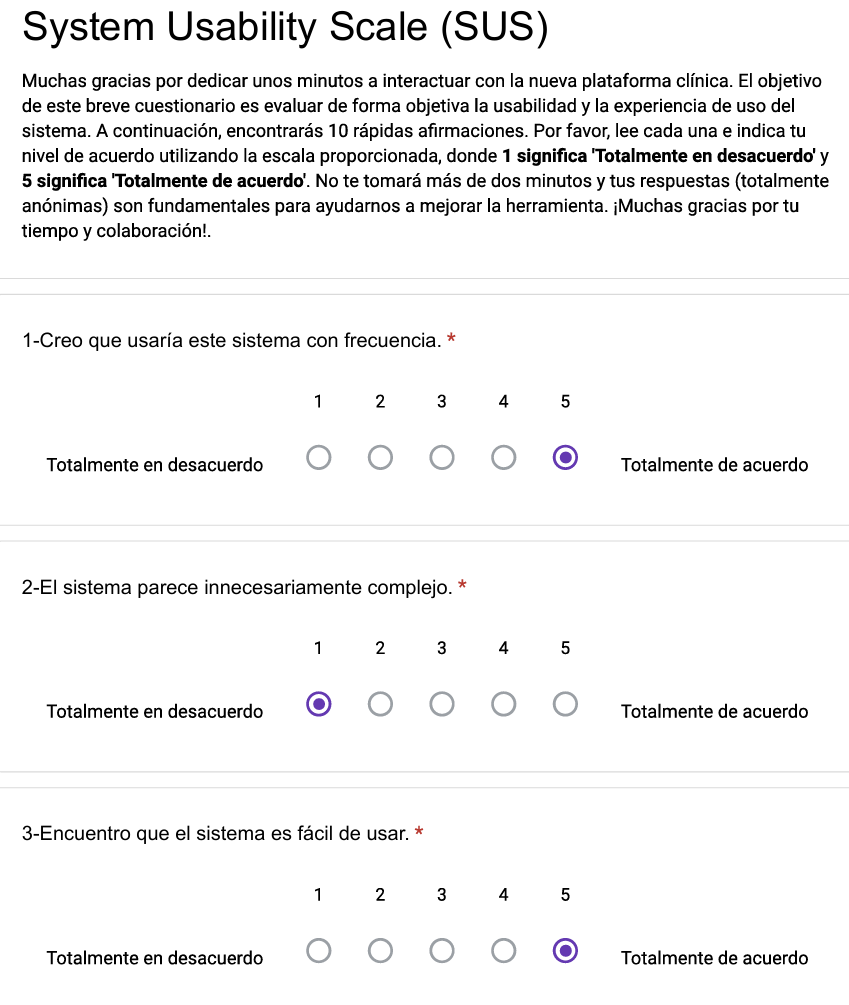
\includegraphics[width=0.5\textwidth]{img/test_a.png}
    	\caption{Respuesta SUS.}
    	\label{fig:test_a}
\end{figure}

\begin{figure}[hbt!]
    	\centering
    	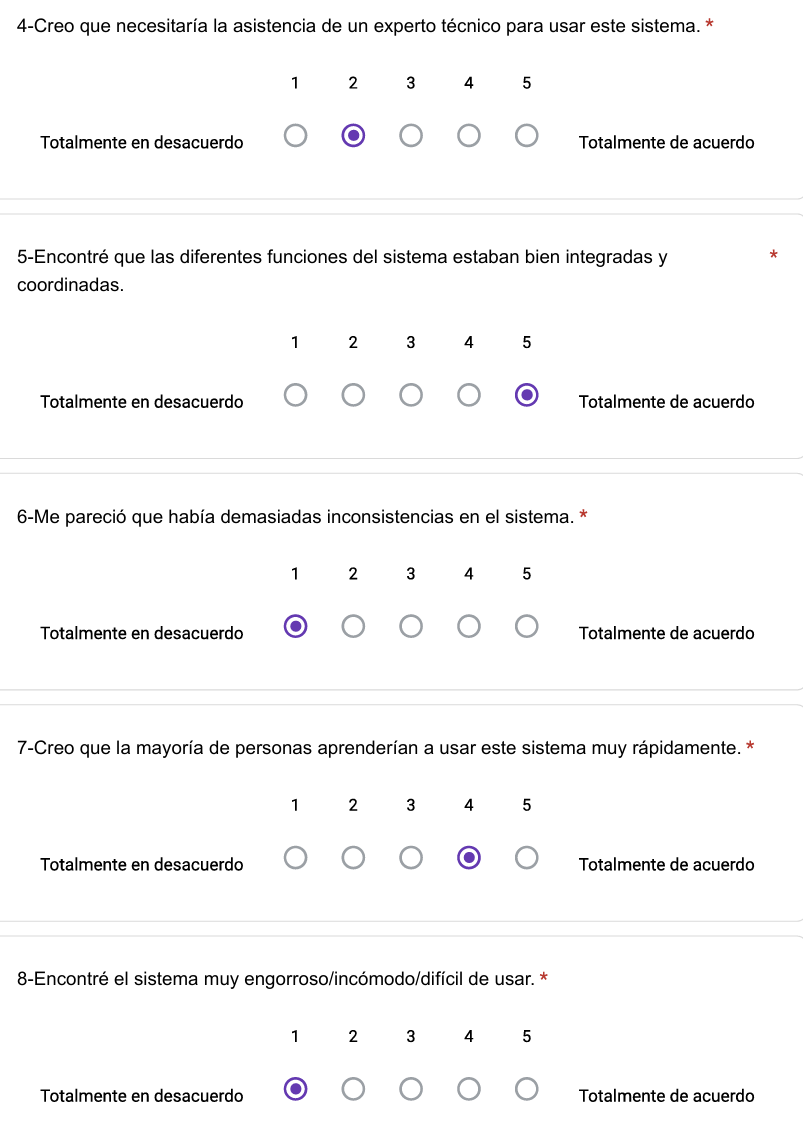
\includegraphics[width=0.5\textwidth]{img/test_b.png}
    	\caption{Respuesta SUS.}
    	\label{fig:test_b}
\end{figure}

\begin{figure}[hbt!]
    	\centering
    	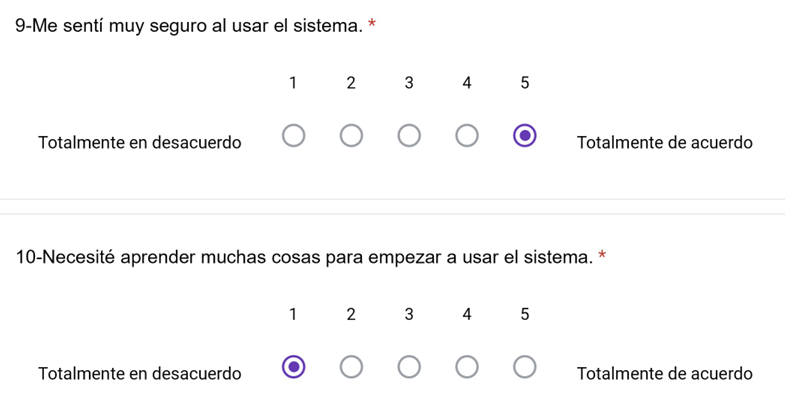
\includegraphics[width=0.5\textwidth]{img/test_c.png}
    	\caption{Respuesta SUS.}
    	\label{fig:test_c}
\end{figure}

Dando en consecuencia el siguiente resultado:

\begin{center}
    \textbf{Puntuación SUS} = ((4+4+4+3+4) + (4+3+4+4+4)) x 2.5 = \textbf{95 / 100}
\end{center}

Este valor supera de forma sobresaliente el umbral de referencia (68) establecido para considerar que una interfaz es aceptable, confirmando que la curva de aprendizaje es mínima y que la aplicación web cumple de forma excelente con su propósito en un entorno hospitalario.

\subsection{Validación Visual y Formatos de Salida}
En paralelo a la usabilidad, se validó la correcta representación de las diferentes herramientas de renderizado de la plataforma. La transformación de los datos en formatos visuales legibles es fundamental para agilizar la toma de decisiones del facultativo. 

A continuación, se exponen los resultados visuales de los módulos de análisis:

\begin{itemize}
    \item \textbf{Visualización Individual de Indicadores (Figura \ref{fig:grafico_individual}):} Renderización de la gráfica de tendencias con su respectivo pasillo de confianza estadístico.
    
    \begin{figure}[hbt!]
    		\centering
    		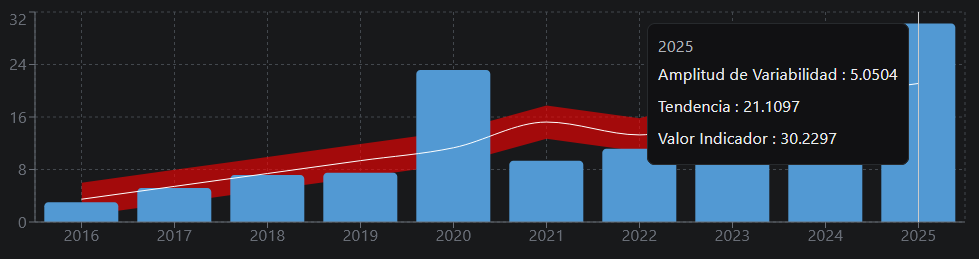
\includegraphics[width=1\textwidth]{img/grafico_individual.png}
    		\caption{Gráfico individual.}
    		\label{fig:grafico_individual}
	\end{figure}
    
    \item \textbf{Herramienta de Mezcla Interactiva (Figura \ref{fig:grafico_mezcla}):} Ejecución del lienzo de correlación, demostrando la capacidad del sistema para superponer hasta tres indicadores distintos simultáneamente. Esta vista permite a los médicos cruzar variables complejas visualmente.
    
    \begin{figure}[hbt!]
    		\centering
    		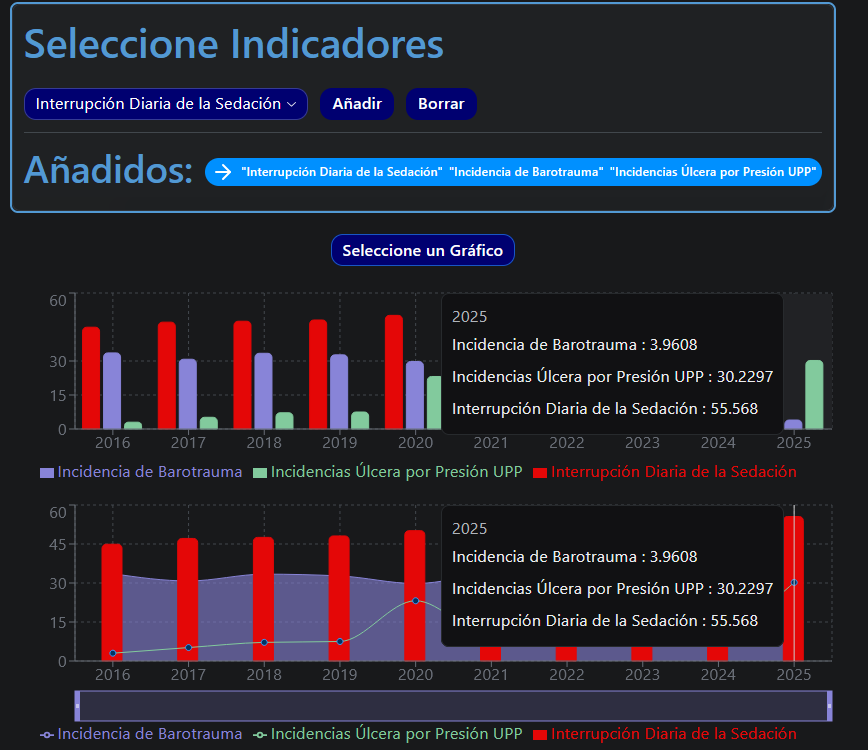
\includegraphics[width=1\textwidth]{img/grafico_mezcla.png}
    		\caption{Correlación de tres indicadores.}
    		\label{fig:grafico_mezcla}
	\end{figure}
    
	\item \textbf{Panel de Resumen Global (Figura \ref{fig:grafico_resumen}):} Condensación de todos los indicadores calculados durante la sesión en formato tabular. Ofrece una radiografía instantánea del estado de la unidad de Reanimación.
	
	\begin{figure}[hbt!]
    		\centering
    		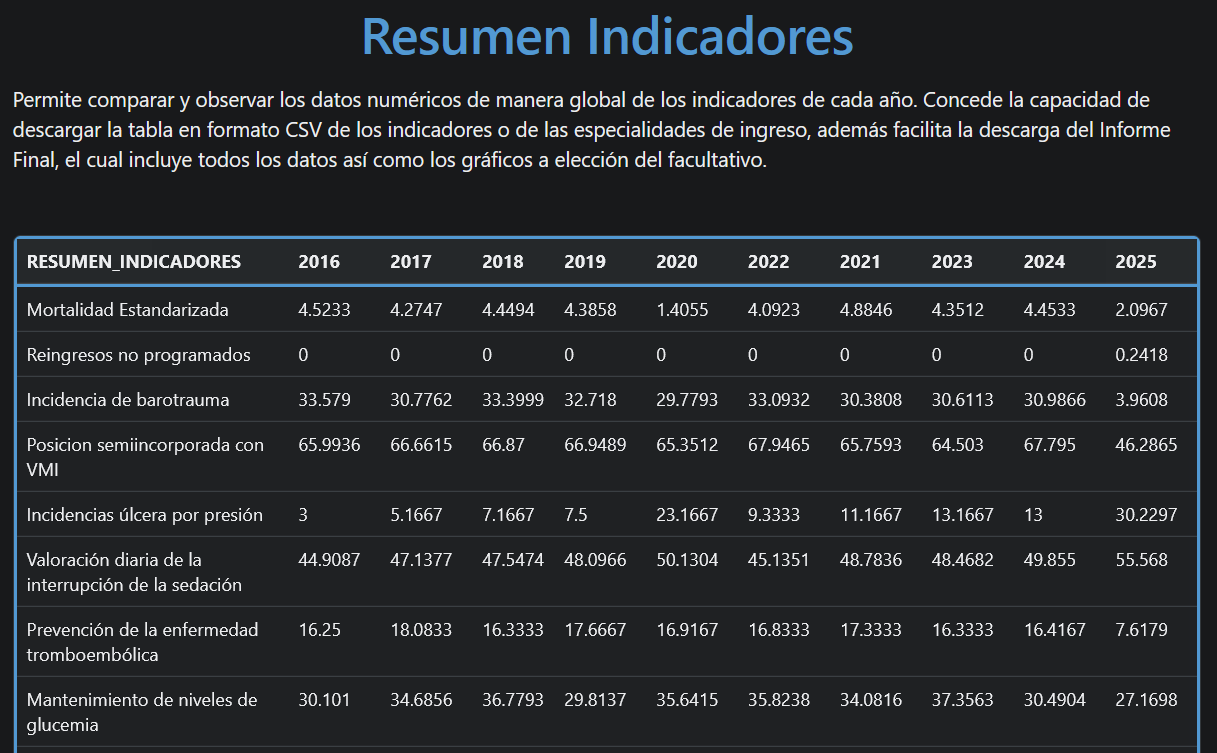
\includegraphics[width=1\textwidth]{img/grafico_resumen.png}
    		\caption{Resumen tabular de los indicadores calculados.}
    		\label{fig:grafico_resumen}
	\end{figure}    
    
    \item \textbf{Generación del Informe Final (Figura \ref{fig:grafico_informe}):} Consolidación automática de los cálculos, textos descriptivos y gráficos generados en la sesión en un documento estructurado en formato \textit{PDF}. El motor aplica de forma automática la regla de las 2 \textit{Sigmas} para colorear en rojo o verde aquellos eventos centinela que se desvían de la media histórica. Constituye el entregable final del sistema, diseñado para su archivo directo en las actas de calidad del hospital.
    
	\begin{figure}[hbt!]
    		\centering
    		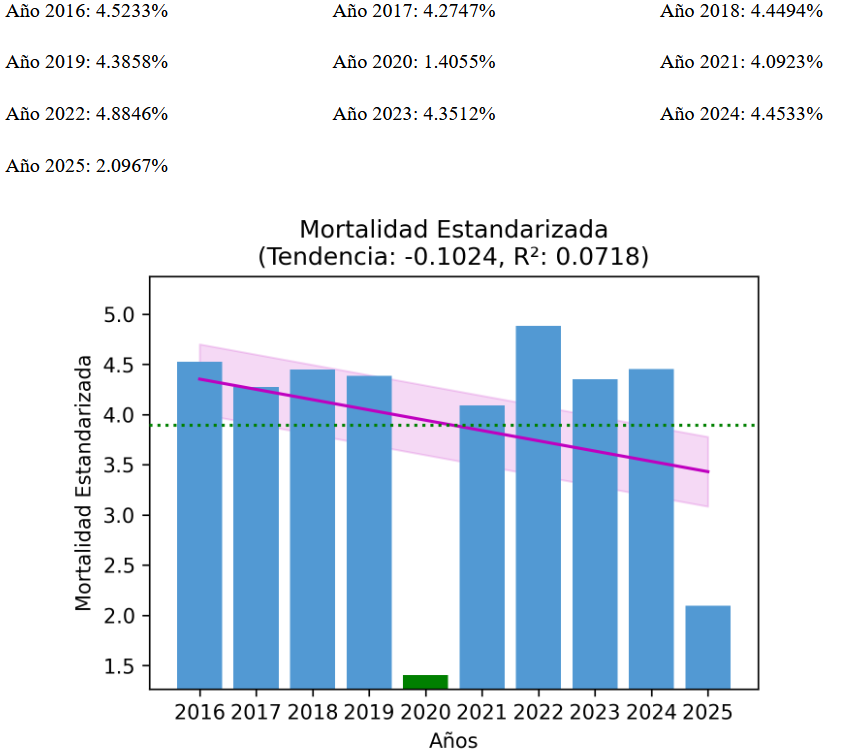
\includegraphics[width=1\textwidth]{img/grafico_informe.png}
    		\caption{Gráfico poseedor de la regla de las 2 \textit{Sigmas} incrustado en el informe final.}
    		\label{fig:grafico_informe}
	\end{figure}    
    
\end{itemize}